\documentclass[11pt]{article}
\usepackage[a4paper,left=1in,right=1in,top=1in,bottom=1in]{geometry}

\usepackage[english]{babel}
\usepackage[T1]{fontenc}
\usepackage[utf8]{inputenc}
\usepackage{seqsplit}

\renewcommand{\familydefault}{\sfdefault}
\usepackage{setspace}  \singlespacing
\usepackage{graphicx}
\usepackage[absolute]{textpos}
\usepackage{xcolor}
\usepackage{fontawesome5}
\usepackage{multirow}
\usepackage{hyperref}
\usepackage{tcolorbox}
\hypersetup{
    colorlinks,
    linkcolor={red!50!black},
    citecolor={blue!50!black},
    urlcolor={blue}
}

\definecolor{mgray}{gray}{0.85}
\definecolor{mpurple}{HTML}{68236D}
\usepackage{float}
\usepackage{subfig,wrapfig}
\usepackage{amsmath,amsfonts,amsthm,amssymb}
\usepackage{fancyhdr,fancybox,color}
\usepackage{enumerate}
\usepackage[amssymb]{SIunits}
\definecolor{MyBlue}{rgb}{0,0.3,0.6}
\usepackage[all]{hypcap}
\usepackage{csquotes}
\usepackage[url=false,
backend=bibtex,
style=authoryear-comp,
doi=true,
isbn=true,
backref=false,
dashed=false,
maxcitenames=2,
maxbibnames=99,
natbib=true]{biblatex}
\DeclareNameAlias{author}{family-given}
\renewbibmacro{in:}{}
\addbibresource{../_logosAndRef/references.bib}
\nonfrenchspacing

\newlength{\headertobodysep}
\setlength{\headertobodysep}{1cm}

\begin{document}
\thispagestyle{empty}

\textblockorigin{0pt}{0pt}

\begin{textblock*}{5cm}(0.5cm,1cm)
    
\includegraphics[height=2cm]{../_logosAndRef/Durham-University.pdf}
\end{textblock*}

\begin{textblock*}{9cm}(6cm,1.5cm)
    \centering
    {\large \textbf{Adhesion vs. Capillarity | CoMPhy Lab}}\\[0.2em]
    Department of Physics, Durham University\\[0.3em]
    \href{https://comphy-lab.org}{comphy-lab.org}
\end{textblock*}

\begin{textblock*}{5cm}(15.5cm,1cm)
    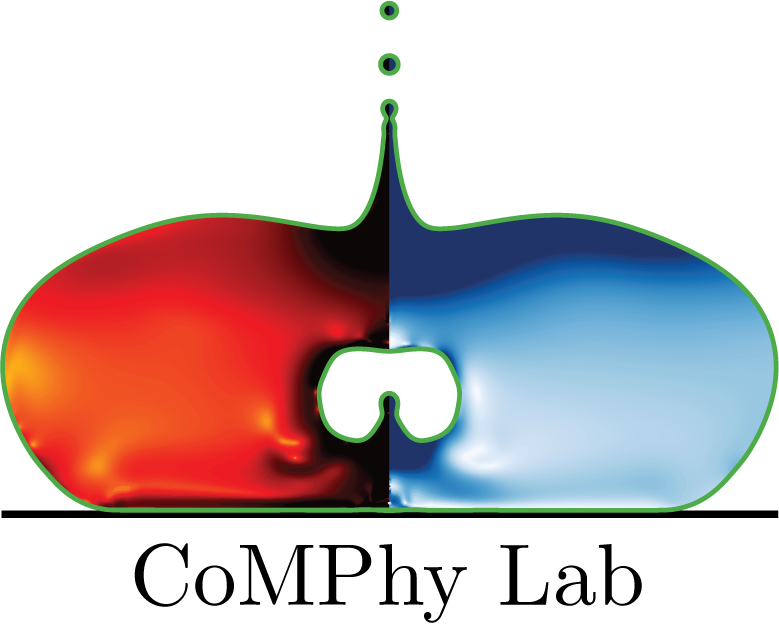
\includegraphics[height=2cm]{../_logosAndRef/CoMPhy-Lab.png}
\end{textblock*}

\vspace*{\headertobodysep}

\begin{center}
    \begin{LARGE}
     When a drop has to choose:\\ adhesion, capillarity, and the physics of wet contact
    \end{LARGE}
\end{center}

\noindent Picture two smooth solids, a wetting fluid film pinned between them at a prescribed contact radius, one solid pulled away from the other at a controlled speed. As the gap opens and the bridge necks, three terms act against the pulling force: a capillary contribution from the curving bridge and a short-range molecular adhesion between the solids, both pulling the surfaces back together, plus a viscous suction that resists the opening motion itself and adds to either attractive term on pull-off. Which term wins sets whether the surfaces snap clean, drain a thin film, or trail a capillary bridge. A textbook account parametrises the contest with two dimensionless groups, a capillary number and an adhesion number, and draws a tidy two-axis regime map. This project argues that picture is incomplete: the gap-to-radius ratio, a stiffness ratio that separates soft JKR-type contact (pull-off by crack propagation at the contact edge) from stiff DMT-type contact (pull-off by uniform adhesive stress across the whole patch) at the same adhesion energy, and a Weissenberg or elastocapillary compliance for non-Newtonian mucus and compliant pads, each enter as essential extra axes, and the biological systems that exploit this contest sit at points no single pair of axes can distinguish. You will build a first-principles theoretical picture of the full parameter space, run axisymmetric Basilisk simulations, and place a curated set of biological attachment systems on the resulting map.

\begin{tcolorbox}[colback=mgray,colframe=mpurple,title=TL;DR]
On pull-off, surface tension and molecular adhesion both pull the surfaces back together; viscosity resists the opening motion and, at fast pull-off, its suction can dominate either attractive term. The outcome is not fixed by a single pair of dimensionless groups. At a minimum you need four: the capillary number $\mathrm{Ca} = \eta U / \gamma$, an adhesion number $\mathrm{Ad} = W_{\mathrm{adh}}/\gamma$, a gap-to-radius ratio $h/R$, and a stiffness ratio $\mu_T$ --- the Tabor number in the Maugis formulation of sphere adhesion --- that sets whether pull-off is the soft JKR limit (a crack peeling back at the edge of the contact patch) or the stiff DMT limit (a uniform attractive layer across the whole patch) at the same adhesion energy~\citep{maugis1992adhesion}. For non-Newtonian exemplars (frog and chameleon tongues) a Weissenberg number $\mathrm{Wi}$ enters; for compliant substrates (torrent-frog toe pad, insect tarsus) an elastocapillary compliance $\gamma/(ER)$ enters. You will derive the limiting scaling laws, run axisymmetric Basilisk simulations of a liquid bridge with a pinned contact line and a disjoining-pressure closure for solid--solid adhesion, sweep the regime plane, and place a curated set of biological attachment systems --- chameleon tongue, torrent frog, clingfish suction, octopus sucker, tree-frog toe pad --- as quantitative markers.
\end{tcolorbox}

\section*{Description}

Why is a tree frog so hard to peel off a vertical pane of glass? Next door, a gecko outdoes the frog dry: a tokay of about 50\,g carries well over forty times its body weight on near-vertical glass, with nothing between its feet and the pane~\citep{autumnGeckoSeta2000}. The frog manages a comparable feat by the opposite route --- a thin wetting film pinned between toe pad and glass. Two different physics, the same qualitative outcome. This project is about the wet side of that dichotomy: what sets the force to pull two wet surfaces apart when there is no muscle and no active suction pump, only surface tension, molecular adhesion, and viscosity.

Two smooth solids are held across a thin wetting film, pinned at a prescribed contact radius; one is withdrawn at a controlled speed. The film thins, the bridge necks, and the force opposing separation is never single-valued. A thin liquid bridge between the surfaces pulls them together with a capillary contribution of order $\gamma R$, where $\gamma$ is surface tension and $R$ the contact radius; opening that gap at rate $\dot h$ generates a Stefan-like viscous suction $F_{\mathrm{visc}} \sim \eta R^4 \dot h / h^3$~\citep{stefan1874} that resists the motion; if the starting film is thin enough for van der Waals forces to bridge the gap, solid--solid attraction adds $F_{\mathrm{vdW}} \sim A R / D^2$ set by the Hamaker constant $A$ and the residual separation $D$. Which term dominates depends on the speed of separation, the viscosity of the intervening fluid, the surface energy, \emph{and} the geometry itself. Textbook treatments collapse the problem onto the two-axis $(\mathrm{Ca}, \mathrm{Ad})$ plane with $\mathrm{Ca} = \eta U/\gamma$ and $\mathrm{Ad} = W_{\mathrm{adh}}/\gamma$. That is the right starting point, but not the right ending point: the crossovers that matter biologically do not obey a universal $(\mathrm{Ca}, \mathrm{Ad})$ diagram.

Three extra dimensionless groups show up the moment you try to place living systems on the map. First, the gap-to-radius ratio $h/R$. The capillary-to-viscous crossover of a pendular bridge has the form $\mathrm{Ca}_\times \sim (h/R)^3 \cos\theta$: at $h/R = 10^{-2}$ it sits eight orders of magnitude below $\mathrm{Ca}_\times$ at $h/R = 1$. Any diagram that projects this out is lying about biology. Second, a stiffness ratio --- the Tabor number $\mu_T = \left[RW_{\mathrm{adh}}^2/(E^{*2} z_0^3)\right]^{1/3}$ in the Maugis formulation of sphere adhesion~\citep{maugis1992adhesion} --- compares how far a compliant contact deforms elastically under its own adhesion energy against the microscopic range over which the adhesive forces themselves act. At large $\mu_T \gtrsim 5$ the contact is soft: adhesion concentrates in a narrow peel-back neck at the edge of the patch and pull-off is set by crack propagation (the JKR limit). At small $\mu_T \lesssim 0.1$ the contact is stiff: adhesion acts as a uniform attractive layer across the whole patch and pull-off is a force balance (the DMT limit). Substituting the same $W_{\mathrm{adh}}$ on two substrates of different $E^*$ gives regime diagrams that look identical on $(\mathrm{Ca}, \mathrm{Ad})$ but behave in opposite limits on $\mu_T$. Third, for the non-Newtonian exemplars (frog and chameleon tongue mucus), a Weissenberg number $\mathrm{Wi} = \dot\gamma\tau$ of order $10^2$ is not a cosmetic addition: a single $\mathrm{Ca}$ evaluated at the Newtonian shear viscosity is simply meaningless, and any pick-and-release design inferred from it will be wrong. For compliant substrates (torrent-frog toe pad, insect tarsus), an elastocapillary compliance $\gamma/(ER) \sim 0.1$--$0.6$ changes the pull-off exponent away from the rigid limit. The full parameter space is at least four-dimensional, and the project's first task is to treat it that way. We therefore ask: across $(\mathrm{Ca}, \mathrm{Ad}, h/R, \mu_T)$, where do the crossovers between capillarity-, viscosity-, and adhesion-dominated pull-off sit, and which of those crossovers do biological attachment systems actually exploit?

Nature has engineered distinguishable points in that space. The chameleon launches its tongue at prey in $\sim 20$\,ms with a viscoelastic mucus film; the mechanism is dominated by viscous adhesion of that film, not by suction, and the Brau et al. analysis places the system at $\mathrm{Ca} \approx 6$ with a pronounced Weissenberg contribution~\citep{brauChameleonTongue2016}. Frog tongues operate similarly but slower~\citep{noelHuFrogTongue2017}. Torrent frogs of the Rhacophoridae use hexagonal toe-pad microchannels to drain excess water at very low pull-off speeds, $\mathrm{Ca} \sim 10^{-5}$--$10^{-3}$, so that the residual film acts as a boundary-friction mediator rather than a capillary trap~\citep{barnesTreeFrogToePads2007,drotlefRockFrogToePad2015}. Clingfish and remora attach through true suction with sustained hydrostatic underpressures of $20$--$50$\,kPa, a regime no $(\mathrm{Ca}, \mathrm{Ad})$ axis can represent~\citep{wainwrightClingfishSuction2013}. Octopus suckers reach even stronger underpressures, approaching $270$\,kPa, through active muscle-driven volume change in the acetabulum~\citep{smithOctopusSucker1991}. Insect tarsi combine capillary bridges and viscous pinning with compliant-pad mechanics~\citep{dirksFederleInsectAdhesion2011,federleAdhesivePadsHairy2006}. Two systems from the original cast are deliberately cut. The gecko is dry and anisotropic~\citep{autumnGeckoSeta2000}; a scalar $W_{\mathrm{adh}}$ does not describe its attachment, and it sits at the degenerate $\mathrm{Ca} = 0$ axis. The \emph{Nepenthes} peristome is an anti-attachment system (aquaplaning \emph{reduces} adhesion to capture prey)~\citep{bohnFederleNepenthes2004}, so its parameter-space location argues the \emph{opposite} physics to the others --- a useful counterexample, not a regime-map sibling.

The project takes this expanded parametrisation as its scaffold. You will derive the pull-off force in each limit from first principles, compute the crossover curves in $(\mathrm{Ca}, \mathrm{Ad}, h/R, \mu_T)$, run a controlled numerical sweep of a canonical axisymmetric geometry, and place the biological systems as markers. The interesting biology sits at the crossovers, not in any one regime, and the crossovers are curves in four dimensions, not points in two.

%-------------------------------------------------------------------
% FIGURE 1 -- Biology montage (suggested)
% Suggested panels (all available under open licenses or CC-BY; Vatsal
% can replace with higher-quality versions):
%   (a) Frog mid-tongue-projection, catching prey
%       (e.g. Beckman collection image; cite Noel & Hu 2017 for the
%       mechanism)
%   (b) Tree frog toe-pad SEM showing hexagonal microchannels
%       (available via CC-BY in several papers; check Barnes 2007 Fig 1,
%       Drotlef et al. 2015, or an open-access Hylidae SEM)
%   (c) Gecko seta / spatula SEM (Autumn group; several open versions)
%   (d) Insect tarsus with fluid droplets (Dirks & Federle 2011 Fig 1 is CC)
%   (e) Nepenthes peristome close-up (Bohn & Federle 2004 or newer CC image)
% Caption: each organism solves a different balance of (Ca, Ad). The
% frog tongue lives at high Ca (fast projection) and high Ad (peptide
% gluing); the tree frog at intermediate Ca with capillarity-assisted
% wet contact; the gecko at near-zero Ca (dry, van der Waals limit);
% the pitcher plant at low Ad / moderate Ca (aquaplaning).
%-------------------------------------------------------------------
\begin{figure}[H]
    \begin{center}
        % \includegraphics[width=\textwidth]{biology_montage.pdf}
        \fbox{\parbox[b][4cm][c]{0.95\textwidth}{\centering\small\emph{Placeholder for biology montage: frog tongue projection, tree frog toe pad (SEM), gecko seta, insect tarsus, Nepenthes peristome. See in-file comments for sources.}}}
        \caption{Curated biological attachment systems that each probe a distinct region of the $(\mathrm{Ca}, \mathrm{Ad}, h/R, \mu_T, \mathrm{Wi})$ space: chameleon tongue (high $\mathrm{Ca}$, high $\mathrm{Wi}$)~\citep{brauChameleonTongue2016}; torrent-frog toe pad (low $\mathrm{Ca}$, small $h/R$, finite $\gamma/(ER)$)~\citep{barnesTreeFrogToePads2007,drotlefRockFrogToePad2015}; clingfish suction (hydrostatic underpressure)~\citep{wainwrightClingfishSuction2013}; octopus sucker (active-muscle suction)~\citep{smithOctopusSucker1991}; insect tarsus (compliant-pad hairy attachment)~\citep{dirksFederleInsectAdhesion2011,federleAdhesivePadsHairy2006}.}
        \label{fig:biology-montage}
    \end{center}
\end{figure}

The idealisation is deliberate: two rigid solids (with a weakly deformable extension for the compliant-pad cases) bridged by a Newtonian fluid, with solid--solid adhesion closed by a disjoining-pressure potential whose energy integral matches $W_{\mathrm{adh}}$. This closure reproduces the JKR and DMT limits as asymptotes, so the Maugis--Dugdale transition appears as an analytical overlay on the simulation sweep rather than a separately resolved contact-mechanics problem. Non-Newtonian exemplars (tongue mucus) and strongly compliant exemplars (toe pads, tarsal pads) are placed on the resulting map from their published rheology and elastic data; they are not re-simulated at the level of constitutive closure in the baseline DNS campaign. No single published study has swept even this idealised setting systematically with modern two-phase tools.

%-------------------------------------------------------------------
% FIGURE 2 -- Schematic of the model problem (to draw in Inkscape/TikZ)
% A vertical axisymmetric section showing:
%   - Upper solid (partial hemisphere or flat punch) with force F upward
%   - Lower solid (flat substrate)
%   - Liquid bridge of minimum neck radius r_n, contact radius a, gap h
%   - Meniscus with contact angle theta_e on each solid
%   - Bulk fluid with viscosity eta, surface tension gamma
%   - Thin solid-solid contact region at centre with adhesion W_adh
% Annotate the three competing forces and the relevant scales.
%-------------------------------------------------------------------
\begin{figure}[H]
    \begin{center}
        % \includegraphics[width=0.8\textwidth]{schematic_bridge.pdf}
        \fbox{\parbox[b][4cm][c]{0.8\textwidth}{\centering\small\emph{Placeholder schematic: axisymmetric liquid bridge between two solids. Annotate $a$, $h$, $\theta_e$, $\gamma$, $\eta$, $W_{\mathrm{adh}}$, applied force $F$.}}}
        \caption{Idealised model problem. Two solids, separated by a wetting liquid bridge, pulled apart at speed $U$. Surface tension $\gamma$, viscosity $\eta$, contact angle $\theta_e$ (pinned at a prescribed radius $a$ on each solid to avoid moving-contact-line singularities), adhesion energy $W_{\mathrm{adh}}$ delivered through a disjoining-pressure potential $\Pi(h)$ with $\int \Pi\,dh = W_{\mathrm{adh}}$. The Basilisk simulations resolve the full axisymmetric flow, including bridge pinch-off, with a minimum-film constraint $h_{\mathrm{min}}/\Delta_{\mathrm{min}} \geq 8$ and $\mathrm{CFL} \leq 0.1$.}
        \label{fig:schematic}
    \end{center}
\end{figure}

%-------------------------------------------------------------------
% FIGURE 3 -- (Ca, Ad) regime diagram, hand-drawn or TikZ
% Axes: log Ca (x), log Ad (y). Three bounded regions:
%   - Capillary-dominated (low Ca, low Ad): Laplace-bridge pull-off
%   - Viscous-dominated (high Ca, low Ad): Stefan cavity
%   - Adhesion-dominated (any Ca, high Ad): JKR / DMT crossover
% Mark approximate positions of the five biological systems in the montage.
%-------------------------------------------------------------------
\begin{figure}[H]
    \begin{center}
        % \includegraphics[width=0.7\textwidth]{regime_diagram.pdf}
        \fbox{\parbox[b][4cm][c]{0.7\textwidth}{\centering\small\emph{Placeholder regime diagram in $(\mathrm{Ca}, \mathrm{Ad})$ space with three asymptotic regions and biology markers.}}}
        \caption{Target of the project: a quantitative regime diagram in $(\mathrm{Ca}, \mathrm{Ad})$ space at fixed $h/R$ and $\mu_T$, separating capillarity-, viscosity-, and adhesion-dominated pull-off. The capillary-to-viscous crossover obeys $\mathrm{Ca}_\times \sim (h/R)^3 \cos\theta$, so the picture moves materially with $h/R$; the JKR/DMT boundary moves with $\mu_T$. Biological attachment systems from Figure~\ref{fig:biology-montage} are placed as markers at their respective $h/R$ and $\mu_T$. The map is a slice of a four-dimensional regime space, not a universal two-axis diagram.}
        \label{fig:regime}
    \end{center}
\end{figure}

\section*{What you will do and what you will learn?}

The project has four scientific objectives --- (i) derive the asymptotic scaling laws and locate the crossover curves; (ii) run a controlled two-phase DNS campaign against those limits; (iii) diagnose where the simple scalings break; (iv) place a curated biological inventory on the resulting map --- plus a craft objective (v) of absorbing the CoMPhy-Lab open-source workflow. Items 1--5 below correspond.

\begin{enumerate}
\itemsep0em
\item Derive the limiting scaling laws from first principles: the Laplace capillary bridge, Stefan-type viscous suction on pull-off~\citep{stefan1874} with the correct $h/R$ dependence, and the JKR/DMT/Maugis--Dugdale adhesion transition~\citep{maugis1992adhesion} parametrised by the Tabor--Maugis number $\mu_T$. Locate the crossover curves $\mathrm{Ca}_\times(h/R)$ and the JKR--DMT boundary in $\mu_T$, rather than assuming they collapse onto a single universal two-axis diagram.
\item Set up axisymmetric two-phase direct numerical simulations in Basilisk C~\citep{popinet2015quadtree} of a liquid bridge between two solids pulled apart at controlled velocity. Pin the contact line at a prescribed radius using Basilisk's contact-angle framework to eliminate the moving-contact-line singularity (no slip model required in the pinned regime); close solid--solid adhesion through a disjoining-pressure potential $\Pi(h)$ with $\int \Pi\,dh = W_{\mathrm{adh}}$; enforce $h_{\mathrm{min}}/\Delta_{\mathrm{min}} \geq 8$ and $h_0/R \geq 0.02$; use $\mathrm{CFL} \leq 0.1$ for the capillary-dominated sweeps. Follow the CoMPhy-Lab two-phase convention~\citep{basiliskVatsal}.
\item Sweep the full $(\mathrm{Ca}, \mathrm{Ad}, h/R, \mu_T)$ space on a coarse grid, measure pull-off force and rupture dynamics, and compare with the analytical limits. Focus on where the simple scalings fail --- at the capillary/viscous crossover $\mathrm{Ca}_\times \sim (h/R)^3 \cos\theta$, at the JKR/DMT transition, and where a disjoining closure changes the bridge-rupture geometry relative to a pure-capillary closure.
\item Place a curated set of biological attachment systems on the regime map --- chameleon tongue~\citep{brauChameleonTongue2016}, frog tongue~\citep{noelHuFrogTongue2017}, torrent-frog toe pad~\citep{barnesTreeFrogToePads2007,drotlefRockFrogToePad2015}, clingfish suction~\citep{wainwrightClingfishSuction2013}, octopus sucker~\citep{smithOctopusSucker1991}, and insect tarsus~\citep{dirksFederleInsectAdhesion2011,federleAdhesivePadsHairy2006} --- treating the Weissenberg number for the non-Newtonian cases and the elastocapillary compliance $\gamma/(ER)$ for the compliant-pad cases as \emph{placement axes}: systems are positioned on the four-dimensional map using their published rheology and elastic data, with $\mathrm{Wi}$ and $\gamma/(ER)$ handled through analytical extensions rather than resimulated at the level of constitutive closure in the baseline DNS campaign. Identify which systems share a regime and which sit at genuinely novel crossovers, and explain why the gecko (dry, anisotropic) and \emph{Nepenthes} (anti-attachment) cannot sit on this map as scalar-$W_{\mathrm{adh}}$ markers.
\item Learn the full open-source workflow of the CoMPhy Lab: Basilisk setup, adaptive mesh refinement, post-processing in Python, documentation via GitHub, and writing for a physics audience~\citep{basiliskVatsalDropFilm,basiliskVatsalViscousBouncing}.
\end{enumerate}

If you have any questions, feel free to contact us \href{mailto:vatsal.sanjay@comphy-lab.org}{vatsal.sanjay@comphy-lab.org}/\\\href{mailto:vatsal.sanjay@durham.ac.uk}{vatsal.sanjay@durham.ac.uk} or drop by Ph255 (Rochester building) at the Department of Physics at Durham University.

\begin{center}
\begin{tabular}{|l|l|l|}
\hline \textbf{Collaborators} & \textbf{E-mail} & \textbf{Based at} \\
\hline \multirow{2}{*}{Dr. Vatsal Sanjay} & \href{mailto:vatsal.sanjay@comphy-lab.org}{vatsal.sanjay@comphy-lab.org} & \multirow{2}{*}{Ph255 (Rochester building)} \\
& \href{mailto:vatsal.sanjay@durham.ac.uk}{vatsal.sanjay@durham.ac.uk} & \\
\hline Dr. Utkarsh Jain & \href{mailto:utkarsh.jain@imec.be}{utkarsh.jain@imec.be} & imec, Leuven \\
\hline
\end{tabular}
\end{center}

\vspace{1em}
\noindent\textit{Last updated: \today}

\printbibliography

\end{document}
